\subsubsection{Over-Regularization}
\label{sxn:underfitting}

%\michael{Is the idea that this section parallels Section~\ref{sxn:Traps}, in that both describe non-\Ideal learning?  If so, we need to refine.  Are we saying that the primarily way $\alpha<2$ is when one layer is compensating for another.  }

The second way we identify $\mathbf{W}$ as \ATypical is when it has an anomalously large variance $(\sigma^2(\WMAT))$.
\michaeladdressed{Variance of what.}

The \SETOL theory -- a single-layer theory of learning -- casts the training 
of a NN layer in terms of how the correlations concentrate into the layer  \EffectiveCorrelationSpace (\ECS),
and becomes exact when the \TRACELOG condition is satisfied.
Analogously, the \HTSR theory -- a single layer \Phenomenology of learning -- casts training
of an N layer by fitting its ESD to a PL, and noting that the PL exponent $\alpha$ measures
the amount of implicit regularization in the layer.
Comparing the two approaches, we see that smaller $\alpha$ corresponds to the correlations
concentrating into a low-rank~\ECS.  In general, and likewise, the more the weight matrix
correlations concentrate  into a low-rank~\ECS, the better the layer has been regularized.
A natural question arises then, namely, can a layer be \emph{\OverRegularized} and
can we detect this?
and in large,
Empirically, we do indeed observe that over the course of training, $\alpha$ decreases, (See Figure~\ref{fig:mlp3-FC1-alpha-overloaded} 
(a), Section~\ref{sxn:hysteresis_effect},) and that the models predictions are concentrated into the~\ECS, 
(See Section~\ref{sxn:empirical-effective_corr_space}). Thus, we also interpret $\alpha$ and~\ECS concentration to be 
measures of learning itself, meaning that NNs are self-regularizing~\cite{MM18_TR_JMLRversion}.

Importantly, however, the \HTSR \Phenomenology indicates that \ALPHA usually lies in the Fat-Tailed Universality class,
such that $\alpha\in [2,6]$.  When $\alpha <2$, the ESD is Very Heavy Tailed (VHT), and, also,
this indicates that $\mathbf{W}$ has an anomalously large variance.  That is,  $\mathbf{W}$ is  \ATypical.
Occasionally, but very infrequently, we do observe $\alpha<2$, and in large, production quality models
(like Llama\cite{LLAMA}).
Interestingly, we also observe that, frequently, when the \HTSR $\alpha<2$, the \SETOL \TRACELOG
condition holds fairly well.  This is further explored in Section~\ref{sxn:empirical}

We have applied the \WW tool to have examined dozens
of modern, very large NNs; of particular interest are the so-called Large Language Models
(LLMs) that have revolutionized the field of AI.  To that end, in Fig.~\ref{fig:falcon_vs_llama},
we present the \WW layer \ALPHA metrics for the Falcon-40b and the Llama-65b LLMs.
\footnote{Similar results are found for the larger, more modern Llama models,
and can be found on the ~\WW website\cite{WW}}

\begin{figure}[ht!]
    \centering
    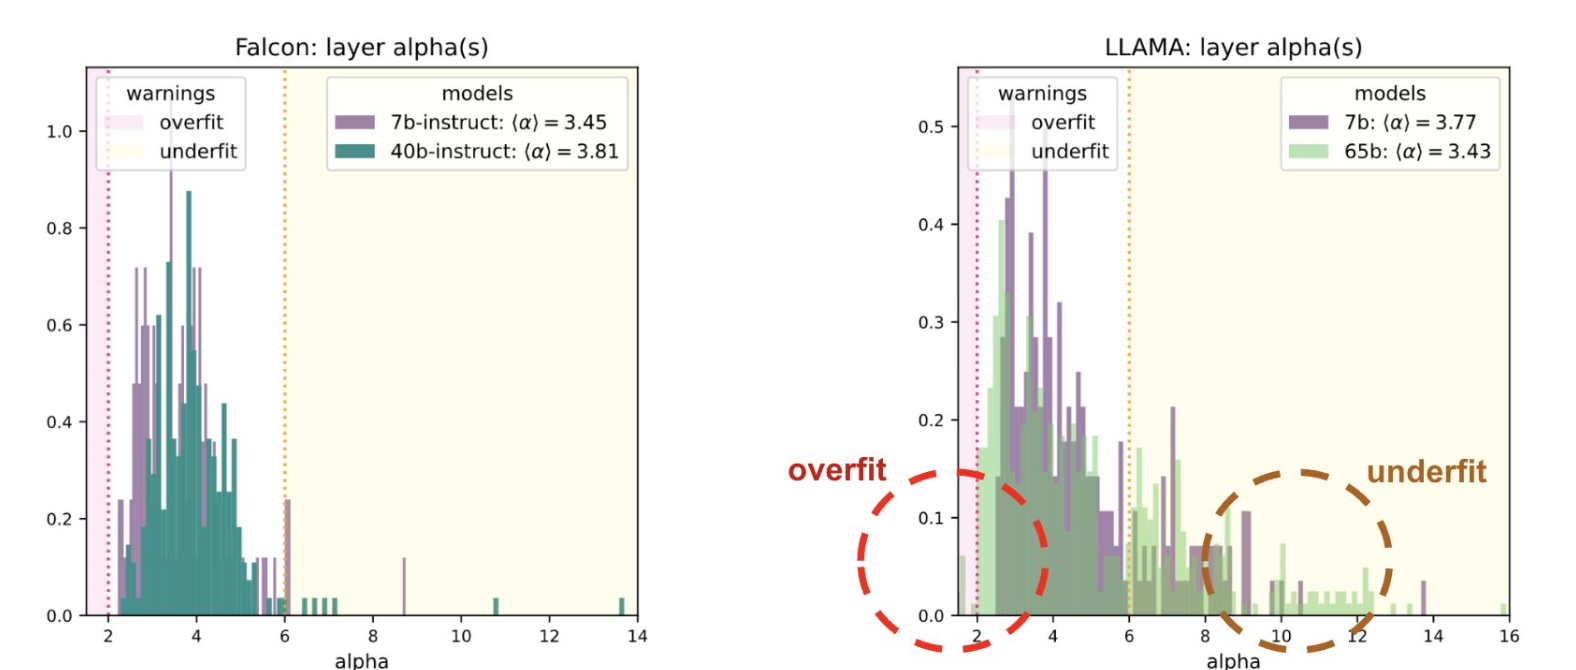
\includegraphics[width=10cm]{./img/falcon_vs_llama.png}
    \caption{Falcon vs Llama}
   \label{fig:falcon_vs_llama}
\end{figure}

For the Falcon-40b model, all of the layer \ALPHA range between $\alpha\in[2,6]$,
and therefore lie in the Fat-Tailed Universality class (in Table~\ref{tab:Uclass})
and are well-fit.
In contrast, looking at the Llama-40b layer \ALPHA, very many have $\alpha>6$,
indicating these layers are under-fit, and while a few have $\alpha <2$, suggesting
these are over-fit.  Finally, there are more layers with $\alpha~\sim2$ in Llama-65
vs Falcon-40b.

The observations on Llama-2 suggest that the layers with $\alpha\le 2$
are compensating for the layers with $\alpha>6$, and yielding suboptimal
performance for the Llama-65b architecture.
Based on these observations, we hypothesize that, in a multi-layer-perceptron (MLP),
when one layer does not or can not learn, then other layers will
have to compensate, and will be overloaded with the training data,
leading to $\alpha<2$, and even the \TRACELOG condition $\Delta \lambda_{min} < 0$.

%In Section~\ref{sxn:empirical} below, we will test this hypothesis in a 3-layer MLP model
%(MLP3), trained on MNIST, but only training 1 (FC1 or FC2), while keeping the other 2 frozen.
%In this way, we can simulate the situation seen above in the Llama-65b model,
%and observe the formation of a HVT ESD in the layer being trained.

%Additionally, as argued below, we conjecture that when $\alpha<2$, the model
%enters a kind-of glassy meta-stable phase, similar to the kinds of phases
%predicted by classic \STATMECH theories of learning.  A
%\nred{explain idea that VHT is \ATypical}

%We will explore how far we can push this analogy in our experiments to stress test the \SETOL approach.
%In particular, we will see effects reminiscent of a glassy system-the slowing down
%of the dynamics (in Sections~\ref{sxn:fc1})
%and a kind of hysteresis (Section~\ref{sxn:hysteresis_effect})

In Section~\ref{sxn:hysteresis_effect}, we will test this hypothesis.
By reducing the trainable parameters in a small MLP, we can simulate the situation seen above in the Llama-65b model,
and observe the formation of a Very Heavy Tailed (VHT) ESD in the dominating layer weight matrix.
Overloading results from having too few parameters for the complexity of the task. Adding more data increases 
the load up to the total complexity of the task itself.
%\st{Adding noisy labels increases the load up to the capacity of the a}

Moreover, we will also argue that in our experiments,
the model enters a kind of glassy meta-stable  phase, similar to the kinds of phases predicted by
classic \STATMECH theories of learning~\cite{SST92}
(described below).
Section~\ref{sxn:hysteresis_effect} will explore how far we can push the analogy of glassy systems in our experiments to 
stress test the \SETOL approach. In particular, we will see effects such as the slowing down of its dynamics, leading to a kind 
of hysteresis, specific to the under-parameterized regime.

